\chapter{Estrutura Analítica de Projetos}\label{apendice-eap}

A estrutura analítica de projetos (EAP) da ferramenta Grasews é apresentada em quatro (4) partes. A \figurename~\ref{fig:grasews-eap-usuario} ilustra os sub-pacotes de trabalho e atividades a fim de entregar o pacote de trabalho denominado \texttt{Usuário}. A \figurename~\ref{fig:grasews-eap-wsdl} ilustra os sub-pacotes de trabalho e atividades a fim de entregar o pacote de trabalho denominado \texttt{WSDL}. A \figurename~\ref{fig:grasews-eap-owl} ilustra os sub-pacotes de trabalho e atividades a fim de entregar o pacote de trabalho denominado \texttt{OWL}. Finalmente, a \figurename~\ref{fig:grasews-eap-colaboracao} ilustra os sub-pacotes de trabalho e atividades a fim de entregar o pacote de trabalho denominado \texttt{Colaboração}.

%\begin{landscape}
    \begin{figure}[h]
        %\resizebox{\textwidth}{!}{
            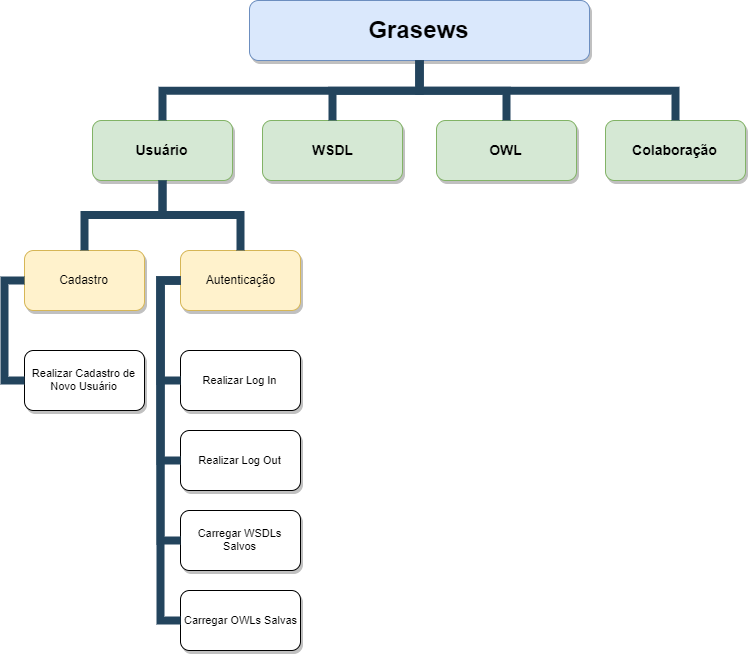
\includegraphics[scale=0.5]{9-pos-textuais/apendices/imagens/grasews-eap-usuario.png}
        %}
        \centering
        \caption[Estrutura Analítica de Projetos de Grasews - Parte 1]{\textbf{Estrutura Analítica de Projetos de Grasews - Parte 1.}}
        \label{fig:grasews-eap-usuario}
    \end{figure}
%\end{landscape}

%\begin{landscape}
    \begin{figure}[h]
        %\resizebox{\textwidth}{!}{
            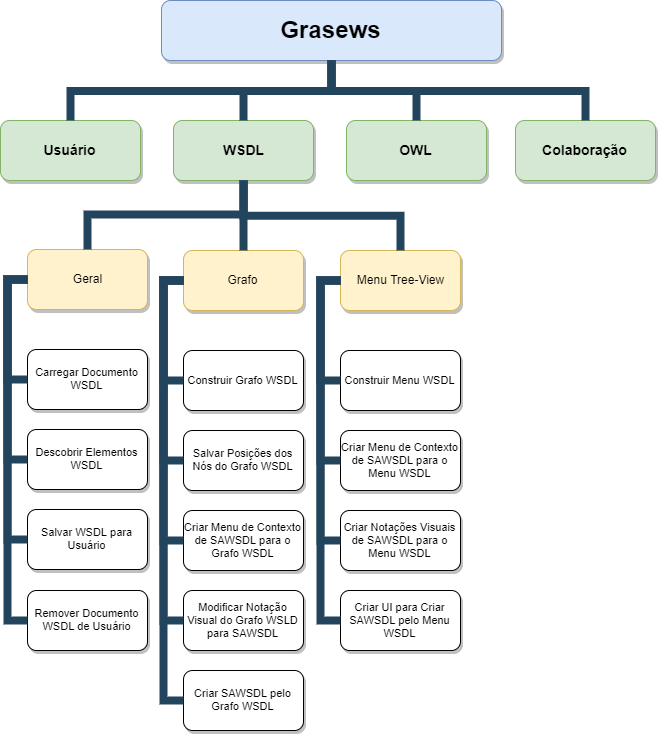
\includegraphics[scale=0.45]{9-pos-textuais/apendices/imagens/grasews-eap-wsdl.png}
        %}
        \centering
        \caption[Estrutura Analítica de Projetos de Grasews - Parte 2]{\textbf{Estrutura Analítica de Projetos de Grasews - Parte 2.}}
        \label{fig:grasews-eap-wsdl}
    \end{figure}
%\end{landscape}

%\begin{landscape}
    \begin{figure}[h]
        %\resizebox{\textwidth}{!}{
            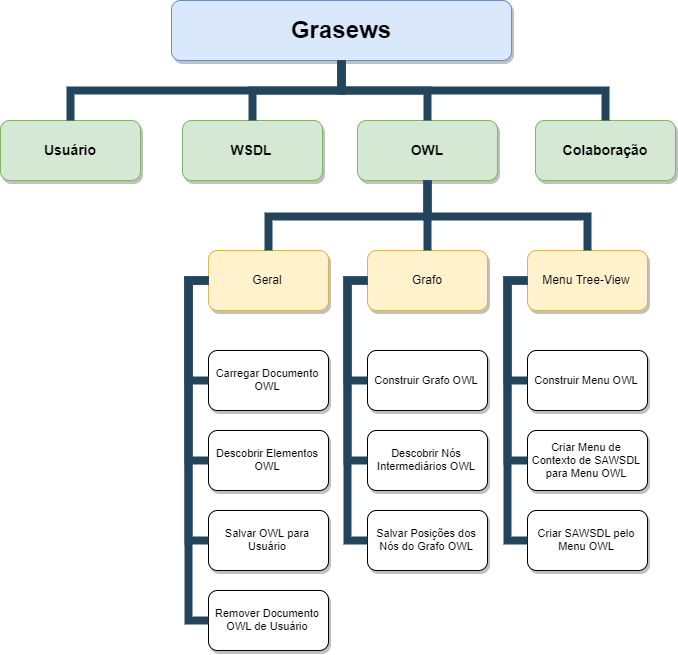
\includegraphics[scale=0.45]{9-pos-textuais/apendices/imagens/grasews-eap-owl.png}
        %}
        \centering
        \caption[Estrutura Analítica de Projetos de Grasews - Parte 3]{\textbf{Estrutura Analítica de Projetos de Grasews - Parte 3.}}
        \label{fig:grasews-eap-owl}
    \end{figure}
%\end{landscape}

%\begin{landscape}
    \begin{figure}[h]
        \resizebox{\textwidth}{!}{
            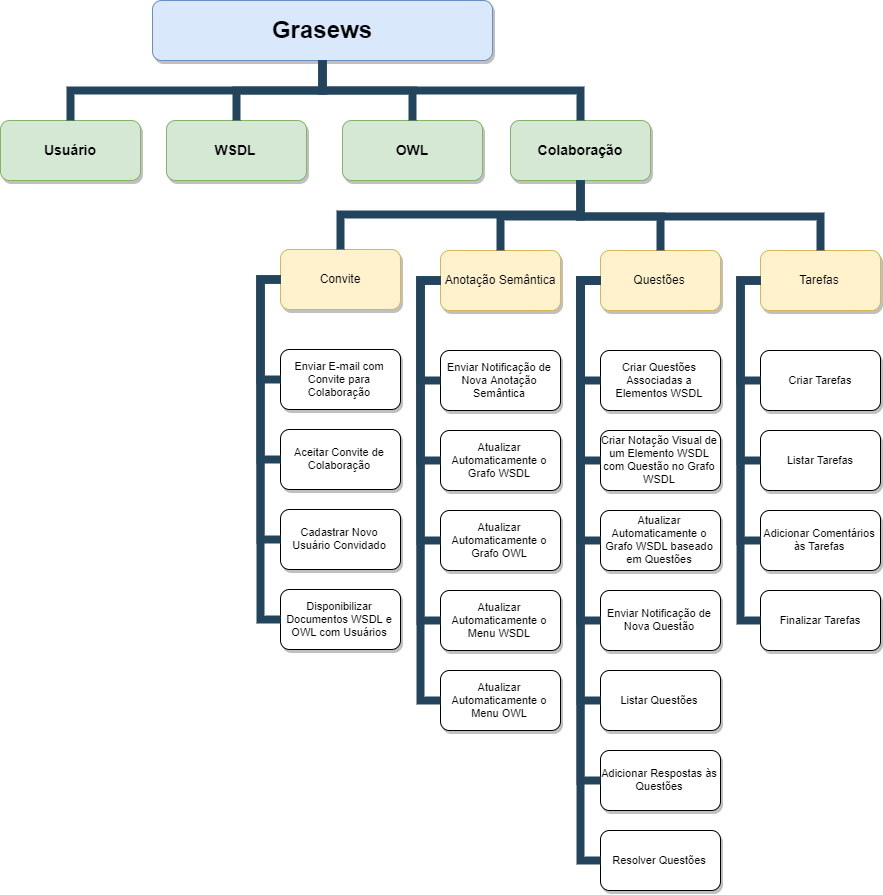
\includegraphics[scale=1]{9-pos-textuais/apendices/imagens/grasews-eap-colaboracao.png}
        }
        \centering
        \caption[Estrutura Analítica de Projetos de Grasews - Parte 4]{\textbf{Estrutura Analítica de Projetos de Grasews - Parte 4.}}
        \label{fig:grasews-eap-colaboracao}
    \end{figure}
%\end{landscape}